\section{Modelling Tools}
Für die Erstellung von Szenen und Objekten, wurden im wesentlichen Cinema 4D und google SketchUp verwendet. Cinema 4D ist eine 3D-Grafiksoftware der Firma Maxon zum Erstellen von 3D-Modellen. Verwendung fand die Software vorallem für das Erstellen der verschiedenen Szenen und für das Modelieren von eingenen Komponenten wie zum Beispiel die eigene Fahrerkabine. Google SkechUp ebenfalls ein Modelierungstool von Google und unterstützt die Modelle die von Google 3D Warehouse heruntergeladen werden können. Darum wurden diese auch gleich mit google SketchUp bearbeitet. Nachfolgend werden beide Tools beschrieben.
\subsection{Cinema 4D}
\label{cinema4d}
\begin{figure}[H]
\centering 
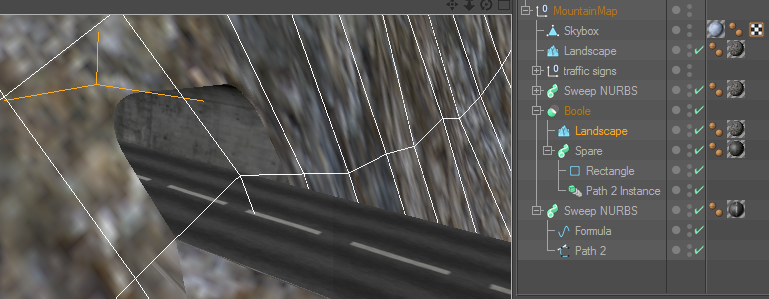
\includegraphics[width=1\linewidth]{src/screenshot_cinema4d.png}
\caption{Screenshot aus Cinema 4D} % Titel der Grafik
\label{screenshot_cinema4d} % Labelname
\end{figure}
\subsection{google SketchUp}\begin{figure}[H]
\centering 
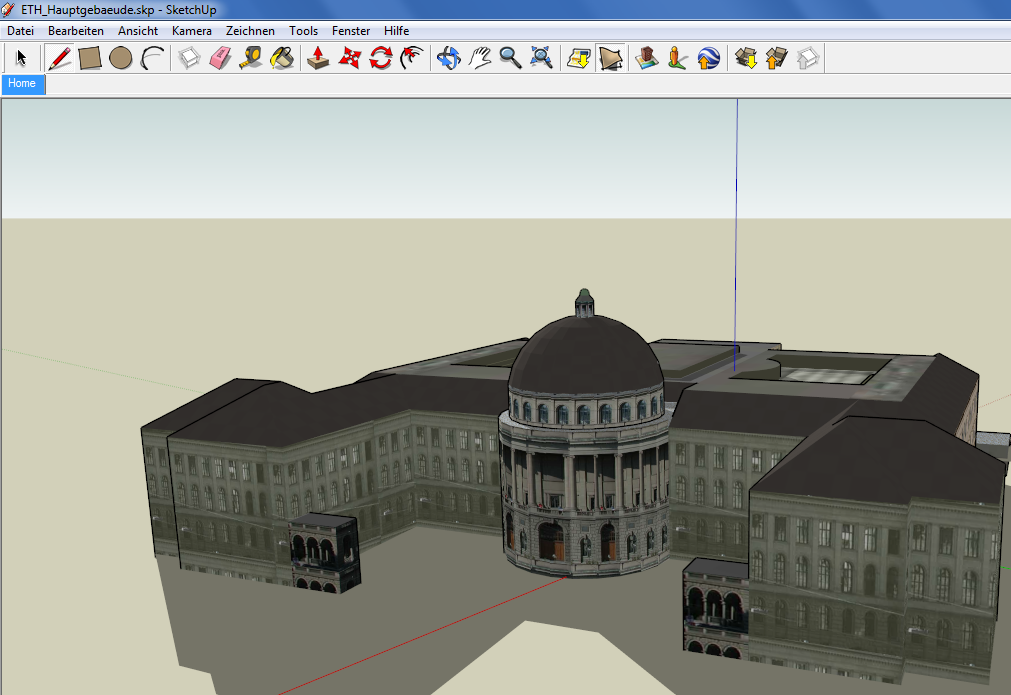
\includegraphics[width=1\linewidth]{src/screenshot_googlesketchup.png}
\caption{Screenshot aus google SketchUp} % Titel der Grafik
\label{screenshot_googlesketchup} % Labelname
\end{figure}